%%
%% CSE407 Final Paper - ACM sigconf format (7-8 page conference version)
%% Target: 7-8 pages
%% Compile: pdflatex -> bibtex -> pdflatex -> pdflatex
%%
\documentclass[sigconf,nonacm]{acmart}

%% -- Extra packages ---------------------------------------------
\usepackage{booktabs}
\usepackage{array}
\usepackage{microtype}
\usepackage{subcaption}
\usepackage{multirow}
\usepackage{float}
\usepackage{placeins}
\usepackage{enumitem}

%% ── Compact Spacing Configurations ─────────────────────────────
\setlist{leftmargin=*,noitemsep,topsep=1.5pt,parsep=0pt,partopsep=0pt}
\setlength{\textfloatsep}{5pt plus 1pt minus 1pt}
\setlength{\floatsep}{4pt plus 1pt minus 1pt}
\setlength{\intextsep}{4pt plus 1pt minus 1pt}
\setlength{\abovecaptionskip}{3pt}
\setlength{\belowcaptionskip}{1.5pt}

%% ── BibTeX compat shim ────────────────────────────────────────
\AtBeginDocument{%
  \providecommand\BibTeX{{Bib\TeX}}%
  \let\balance\relax}

%% ── Remove all conference / copyright metadata ─────────────────
\setcopyright{none}
\acmYear{2026}
\acmDOI{}
\acmConference[]{}{}{}
\acmISBN{}
\settopmatter{printacmref=false}
\setlength{\headheight}{23.5pt}
\setlength{\emergencystretch}{2em}
\raggedbottom

%% ── Macros ─────────────────────────────────────────────────────
\newcommand{\cmark}{\ensuremath{\checkmark}}
\newcommand{\xmark}{\ensuremath{-}}

\begin{document}

%% ════════════════════════════════════════════════════════════════
%%  TITLE AND AUTHORS
%% ════════════════════════════════════════════════════════════════
\title{Multi-Stage Compression of Small Language Models for Energy-Efficient Inference: An Empirical Systems Ablation}

\author{\mbox{}}
\renewcommand{\shortauthors}{}

%% ════════════════════════════════════════════════════════════════
%%  ABSTRACT
%% ════════════════════════════════════════════════════════════════
\begin{abstract}
Deploying small language models (SLMs) on power-constrained hardware requires balancing energy consumption, memory footprint, decode throughput, and task accuracy. Most compression techniques (such as 4-bit weight quantization, token eviction, and KV-cache quantization) are evaluated in isolation, but practical systems stack them sequentially. In this paper, we measure the physical interactions, operating boundaries, and software-to-hardware realization gaps of stacked compression pipelines on an NVIDIA T4 GPU across context lengths of 1024, 2048, and 4096 tokens, logging board power at 10~Hz via NVML. We evaluate retrieval quality using a calibrated 60-scenario hard-retrieval benchmark requiring exact-match key-value extraction from 4096-token documents across three insertion depths.

Our measurements demonstrate that compression efficiency depends directly on attention head layout and sequence length rather than nominal compression ratios alone. On Llama~3.2-3B (3:1 GQA), combining 4-bit AWQ with custom PyramidKV eviction delivers the best overall result at 4096 tokens: total energy decreases by 101.95~J (16.15\%), active KV cache storage drops by 73.8\% (from 455~MiB to 119~MiB), decode throughput increases 47.7\% (from 13.77 to 20.34~tok/s), and retrieval accuracy remains within one test scenario of baseline (37/60 vs.\ 38/60). However, applying the same eviction policy to Qwen2.5-3B (8:1 GQA) collapses retrieval accuracy from 48/60 to 1/60, a failure that persists even after expanding the retained token budget by 50\% (recovering only 2/15). We also measure a statistically significant negative interaction contrast ($I < 0, p < 0.01$), confirming that pruning tokens prior to quantization reduces downstream memory traffic and shields against quantizer runtime overhead. Finally, we document a software-to-hardware realization gap in the TurboQuant reference package, which retains uncompressed tensors alongside discrete indices and increases physical memory by over 50\%. These measurements provide empirical boundary conditions for joint rate-distortion frameworks like ThinKV and RDKV.
\end{abstract}

%% ── CCS Concepts ──────────────────────────────────────────────
\begin{CCSXML}
<ccs2012>
   <concept>
       <concept_id>10010583.10010662.10010668</concept_id>
       <concept_desc>Hardware~Power estimation and optimization</concept_desc>
       <concept_significance>500</concept_significance>
   </concept>
   <concept>
       <concept_id>10010147.10010178.10010179</concept_id>
       <concept_desc>Computing methodologies~Natural language processing</concept_desc>
       <concept_significance>500</concept_significance>
   </concept>
   <concept>
       <concept_id>10010583.10010786</concept_id>
       <concept_desc>Hardware~Memory and dense storage</concept_desc>
       <concept_significance>300</concept_significance>
   </concept>
   <concept>
       <concept_id>10010147.10010257</concept_id>
       <concept_desc>Computing methodologies~Machine learning</concept_desc>
       <concept_significance>300</concept_significance>
   </concept>
</ccs2012>
\end{CCSXML}

\ccsdesc[500]{Hardware~Power estimation and optimization}
\ccsdesc[500]{Computing methodologies~Natural language processing}
\ccsdesc[300]{Hardware~Memory and dense storage}
\ccsdesc[300]{Computing methodologies~Machine learning}

%% ── Keywords ───────────────────────────────────────────────────
\keywords{Green AI, energy-efficient inference, KV cache compression, token eviction, weight quantization, AWQ, TurboQuant, PyramidKV, small language models, edge deployment, NVIDIA T4, needle-in-a-haystack}

\maketitle

%% ════════════════════════════════════════════════════════════════
%%  1. INTRODUCTION
%% ════════════════════════════════════════════════════════════════
\section{Introduction}

Deploying small language models (SLMs) on resource-constrained hardware involves a trade-off between energy consumption, memory footprint, decode throughput, and task accuracy~\cite{strubell_energy_2019,patterson_carbon_2021,schwartz2020green}. The deployment trend of performing inference workloads on local micro-servers and low-power accelerators makes the KV cache's memory bandwidth demand a major operational bottleneck~\cite{li2024survey}.

Transformers retain key and value vectors for each token processed during autoregressive generation, causing the KV cache to grow linearly with sequence length~\cite{li2024survey}. Because each decoded token repeatedly accesses the accumulated cache, inference on bandwidth-limited hardware can become memory bound during decoding~\cite{dao_flashattention_2022}. Small language models with sub-4B parameters provide a practical footprint for resource-constrained deployments~\cite{husom_sustainable_2025}. However, their physical energy scaling under multi-stage compression remains poorly characterized. Most prior compression studies evaluate individual techniques in isolation, rely on theoretical FLOP calculations, or evaluate large server-scale models with attention dynamics that differ from compact SLMs~\cite{wang_slmquant_2025}.

Prior work reduces generation-time memory traffic through three mechanisms. Weight quantization, including AWQ~\cite{lin_awq_2025}, uses low-bit weights to reduce static storage and parameter-transfer bandwidth. Token-eviction methods such as PyramidKV, SnapKV, and H2O~\cite{cai_pyramidkv_2025,li_snapkv_2024,zhang_h2o_2023} prune low-importance cache entries to reduce active memory and decode traffic. KV-cache quantizers such as TurboQuant, KIVI, and JanusQuant~\cite{zandieh2026turboquant,liu_kivi_2023,sun2026janusquant} instead reduce the precision stored per token.

Theoretical frameworks such as RDKV and ThinKV combine token pruning with precision reduction through rate-distortion objectives~\cite{zhang_rdkv_2026,ramachandran_thinkv_2026}. Although these formulations show strong simulated trade-offs, physical hardware data for sub-4B models remains scarce. Practitioners therefore lack empirical evidence about sequentially stacked compression tools, the effect of attention head-sharing on pruning reliability, and deployment-time runtime overhead.

We therefore present an empirical systems study of multi-stage compression interactions on physical silicon. We sequentially measure AWQ 4-bit weight quantization, custom PyramidKV token eviction, and TurboQuant KV-cache quantization on two representative 3B models (Llama~3.2-3B-Instruct and Qwen2.5-3B-Instruct) on an NVIDIA T4 GPU, continuously logging board power at 10~Hz with NVML~\cite{argerich_watt_2026,nvidia2024nvml}.

\paragraph{Research Questions.}
In this study, we investigate four core questions:
\textbf{RQ1 (Context Scaling and Multi-Stage Efficiency):} How do weight quantization, token eviction, and KV-cache quantization affect physical GPU energy consumption and throughput when applied independently and sequentially across 1024, 2048, and 4096 tokens?
\textbf{RQ2 (Cross-Architectural Robustness):} Does token eviction provide consistent trade-offs across different attention layouts (Llama's 3:1 and Qwen's 8:1 GQA) or does aggressive head sharing cause retrieval failures?
\textbf{RQ3 (Compound Interaction and Overhead Shielding):} When multiple compression stages are applied sequentially, do their effects add up or is there an energetic shielding interaction?
\textbf{RQ4 (Multi-Objective Pareto Optimization):} Which compression configurations form the non-dominated Pareto frontier for energy, retrieval accuracy, decode throughput, and persistent memory footprint under bootstrap resampling?

\paragraph{Key Contributions.}
The main empirical discoveries of this work are:
\textbf{(1) Limits of Sequential Stacking:} Stacking independent compression techniques does not compose well in terms of energy on physical hardware. The best performing combination on Llama~3.2-3B (3:1 GQA) was single-stage token eviction + AWQ which demonstrated a 101.95~J (16.15\%) total energy reduction relative to the AWQ baseline, a 47.7\% higher decode speedup (13.77 to 20.34~tok/s), a 73.8\% smaller active KV-cache footprint (455~MiB to 119~MiB), and retrieval accuracy within one test case of baseline (37/60 vs.\ 38/60). Adding sequential quantization decreased throughput while increasing total energy.
\textbf{(2) Attention Head-Sharing Sensitivity:} Eviction heuristics do not transfer reliably across Grouped-Query Attention (GQA) ratios~\cite{ainslie2023gqa}. Using the same eviction heuristic on Qwen2.5-3B (8:1 GQA) reduced retrieval accuracy to only 1/60. Increasing the token budget by 50\% recovered only two additional cases (2/15), showing that tokens were erroneously evicted due to head-sharing patterns rather than insufficient capacity.
\textbf{(3) Upstream Overhead Shielding:} Across both models, we measure substantial negative interaction contrasts ($I < 0, p < 0.01$). Pruning tokens prior to quantization shrinks effective cache volumes by up to 73.8\%, reducing downstream quantizer processing overhead and shielding against runtime overhead.
\textbf{(4) Software-to-Hardware Realization Gaps:} Straightforward deployment of existing quantization libraries can diverge substantially from theoretical expectations. TurboQuant's reference implementation incurs 31\% to 45\% additional energy overhead while incurring large DRAM allocation overheads by retaining uncompressed FP16 tensors alongside discrete indices.

%% ════════════════════════════════════════════════════════════════
%%  2. RELATED WORK
%% ════════════════════════════════════════════════════════════════
\section{Related Work}

\paragraph{Weight Quantization.}
Weight quantization compresses floating-point model parameters to lower-bit integers to reduce static memory consumption and parameter transfer bandwidth. AWQ~\cite{lin_awq_2025} identifies activation-salient weight channels and protects them from quantization errors in 4-bit compression. GPTQ~\cite{frantar_gptq_2023} conducts layerwise error compensation. SLMQuant~\cite{wang_slmquant_2025} found that compact sub-4B models are more sensitive to aggressive quantization than larger models. This sensitivity highlights the necessity of directly evaluating hardware on specific SLMs rather than assuming trends observed in large LLMs carry over.

\paragraph{Token Eviction.}
Token eviction prunes uninformative tokens during generation, which decreases KV-cache memory. H2O~\cite{zhang_h2o_2023} showed that a small fraction of accumulated attention recipients (around 20\%) is enough to maintain most generative capability. SnapKV~\cite{li_snapkv_2024} relies on an observation window on recent prompt positions for important token selection. PyramidKV~\cite{cai_pyramidkv_2025} improves this by introducing layer-dependent budgets, where deeper layers hold more tokens while shallower layers hold fewer, improving long-context retrieval accuracy by 5\% to 15\% compared to uniform budgets.

\paragraph{KV-Cache Quantization.}
KV-cache quantization reduces the numerical precision of stored key and value vectors. TurboQuant~\cite{zandieh2026turboquant} applies random orthogonal rotations on KV vectors and then performs scalar quantization, without requiring calibration data. KIVI~\cite{liu_kivi_2023} employs per-channel key and per-token value quantization with 2-bit precision. Salfati et al.~\cite{salfati_quantization_2026} found that uniform quantization maintains the ranking of attention scores better compared to low-rank approximations, especially for grouped-query attention (GQA) architectures. JanusQuant was proposed by Sun et al.~\cite{sun2026janusquant} for long-context 2-bit quantization.

\paragraph{Joint Compression and Energy Measurement.}
Recent theoretical work combines token pruning with precision reduction. RDKV~\cite{zhang_rdkv_2026} formulates KV-cache compression as rate-distortion optimization using reverse water-filling. ThinKV~\cite{ramachandran_thinkv_2026} employs dynamic token and precision allocation for reasoning models. Argerich et al.~\cite{argerich_watt_2026} analyzed 5,000+ inference runs and demonstrated that 10~Hz NVML power sampling provides accurate, low-overhead GPU energy measurement (recording $\approx 12$~W idle and 82~W peak on NVIDIA T4). Husom et al.~\cite{husom_sustainable_2025} measured quantized SLMs on edge hardware, showing energy scaling depends on sequence length and workload. In our study we combine these measurement protocols to evaluate multi-stage interactions on physical silicon.

\begin{table}[t]
\caption{Coverage Comparison with Related Work}
\label{tab:comparison}
\centering\small
\setlength{\tabcolsep}{5pt}
\begin{tabular}{@{}lcccc@{}}
\toprule
\textbf{Work} & \textbf{Wt.Q} & \textbf{Evict} & \textbf{KVQ} & \textbf{Energy} \\
\midrule
AWQ~\cite{lin_awq_2025}            & \cmark & \xmark & \xmark & \xmark \\
GPTQ~\cite{frantar_gptq_2023}      & \cmark & \xmark & \xmark & \xmark \\
SLMQuant~\cite{wang_slmquant_2025} & \cmark & \xmark & \xmark & \xmark \\
H2O~\cite{zhang_h2o_2023}          & \xmark & \cmark & \xmark & \xmark \\
SnapKV~\cite{li_snapkv_2024}       & \xmark & \cmark & \xmark & \xmark \\
PyramidKV~\cite{cai_pyramidkv_2025}& \xmark & \cmark & \xmark & \xmark \\
TurboQuant~\cite{zandieh2026turboquant} & \xmark & \xmark & \cmark & \xmark \\
KIVI~\cite{liu_kivi_2023}          & \xmark & \xmark & \cmark & \xmark \\
RDKV~\cite{zhang_rdkv_2026}        & \xmark & \cmark & \cmark & \xmark \\
ThinKV~\cite{ramachandran_thinkv_2026} & \xmark & \cmark & \cmark & \xmark \\
Watt Counts~\cite{argerich_watt_2026} & \xmark & \xmark & \xmark & \cmark \\
\midrule
\textbf{This Work}                 & \textbf{\cmark} & \textbf{\cmark} & \textbf{\cmark} & \textbf{\cmark} \\
\bottomrule
\end{tabular}
\end{table}

%% ════════════════════════════════════════════════════════════════
%%  3. METHODOLOGY AND BENCHMARK DESIGN
%% ════════════════════════════════════════════════════════════════
\section{Methodology and Benchmark Design}

Figure~\ref{fig:methodology} illustrates our experimental workflow across model configurations, power profiling, benchmark evaluation, and statistical validation.

\begin{figure}[t]
\centering
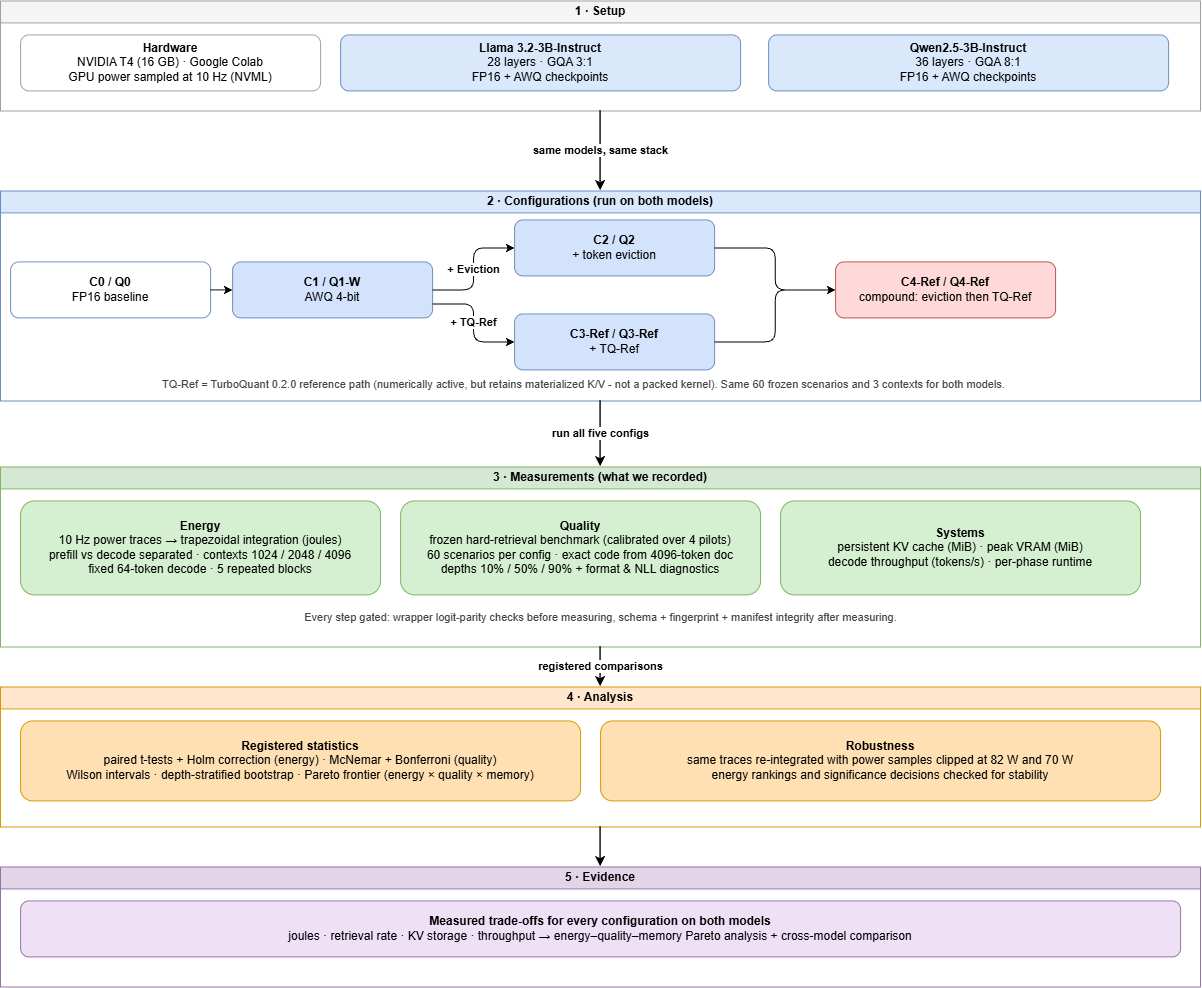
\includegraphics[width=0.72\columnwidth]{figures/methodology_diagram.png}
\Description{Flowchart of the experimental workflow: five compression configurations evaluated on Llama 3.2-3B and Qwen2.5-3B, logging 10 Hz power traces, hard-retrieval quality, and system trade-offs.}
\caption{Experimental workflow for both models, including compression, 10~Hz power logging, retrieval evaluation, and system trade-off analysis.}
\label{fig:methodology}
\end{figure}

\subsection{Model Architectures and Configurations}
We evaluated two 3B-parameter open-weight models: Llama~3.2-3B-Instruct (28 layers, 24 query heads, 8 KV heads, 3:1 GQA ratio~\cite{ainslie2023gqa}, 8K native context) and Qwen2.5-3B-Instruct (36 layers, 16 query heads, 2 KV heads, 8:1 GQA ratio, 32K native context), both using head dimension 128. For Llama, we used the Unsloth FP16 baseline~\cite{unsloth_2024} and CasperHansen AWQ release~\cite{casperhansen_llama32_awq}. For Qwen, we use official Qwen2.5-3B-Instruct checkpoints~\cite{qwen2024technical}. Our software environment runs PyTorch~2.11.0~\cite{paszke2019pytorch}, Transformers~5.12.1~\cite{wolf2020transformers}, and TurboQuant~0.2.0~\cite{zandieh_turboquant_v020}.

We experimented five core configurations: \textbf{(1) FP16 Baseline (C0 / Q0):} Uncompressed execution serving as the reference standard; \textbf{(2) AWQ Baseline (C1-W / Q1-W):} 4-bit weight-only quantization without KV compression to isolate its static parameter savings; \textbf{(3) Eviction (C2 / Q2):} AWQ with layerwise token eviction averaging 1024 retained tokens per layer to reduce decode memory traffic; \textbf{(4) TQ-Ref Only (C3-Ref / Q3-Ref):} AWQ with numerical KV quantization to assess retrieval quality alongside reference runtime overhead; and \textbf{(5) Compound Stack (C4-Ref / Q4-Ref):} Sequential composition (AWQ $\to$ eviction $\to$ TurboQuant) to measure multi-stage interactions.

\subsection{Hardware and Power Measurement Protocol}
All experiments executed on an NVIDIA Tesla T4 GPU (16~GB nominal VRAM, 70~W nominal cap) on Google Colab. We polled GPU board power at 10~Hz (every 100~ms) through NVML~\cite{nvidia2024nvml} using \texttt{pynvml}, following Argerich et al.~\cite{argerich_watt_2026}. Total energy was computed by trapezoidal numerical integration over recorded power traces, separating prefill and decode phases. All energy runs used teacher-forced decoding for exactly 64 tokens to isolate compression effects from open-ended text variation across context lengths of 1024, 2048, and 4096 tokens with five independent measurement blocks per condition ($n=5$).

\subsection{Eviction and TurboQuant Realization Audit}
Token eviction was implemented using a custom PyTorch attention wrapper. During prefill, token importance scores are computed by averaging attention weights over a 32-token observation window. We apply a layer-dependent pyramidal budget averaging 1024 retained tokens per layer (larger budgets in deeper layers, smaller in shallow layers, decay $\beta=20$). Tokens below the threshold are pruned before decoding starts.

TurboQuant~\cite{zandieh2026turboquant} applies random orthogonal rotations to KV vectors and maps coordinates to discrete codebook indices. We evaluate the public reference package (v0.2.0)~\cite{zandieh_turboquant_v020}. In this package, coordinates are stored as \texttt{uint8} indices while uncompressed FP16 key and value tensors remain concurrently allocated in GPU memory. Consequently, the reference path is numerically active during attention computation but does not reduce physical device memory. This provides an empirical audit of the \emph{software-to-hardware realization gap}. A custom packed and fused kernel achieves net energy reduction only when compute overhead remains below the memory traffic boundary: $O_\text{net} < \epsilon_\text{mem} \cdot \Delta_D$, where $\epsilon_\text{mem}$ is energy saved per byte and $\Delta_D$ is avoided decode traffic.

\subsection{Calibrated Hard-Retrieval Benchmark}
\label{sec:benchmark}
Standard downstream NLP benchmarks probe static weights rather than KV-cache degradation, while naive synthetic needle-in-a-haystack (NIAH) benchmarks~\cite{kamradt2023needle} exhibited a 100\% retrieval ceiling effect across all compressed SLM configurations in our preliminary trials. Following KV-cache compression evaluation methodology~\cite{cai_pyramidkv_2025,li_snapkv_2024,zhang_h2o_2023}, we designed a calibrated 4096-token hard-retrieval benchmark requiring exact-match UUID key-value extraction across 60 frozen scenarios (20 at 10\%, 20 at 50\%, and 20 at 90\% document depth), illustrated in Figure~\ref{fig:hard_retrieval}. Distractor density and key distinctiveness were calibrated across four pilot iterations so that uncompressed baselines achieve high but imperfect accuracy ($\approx 75\%-88\%$), providing headroom to detect compression loss without floor or ceiling artifacts.

\begin{figure}[t]
\centering
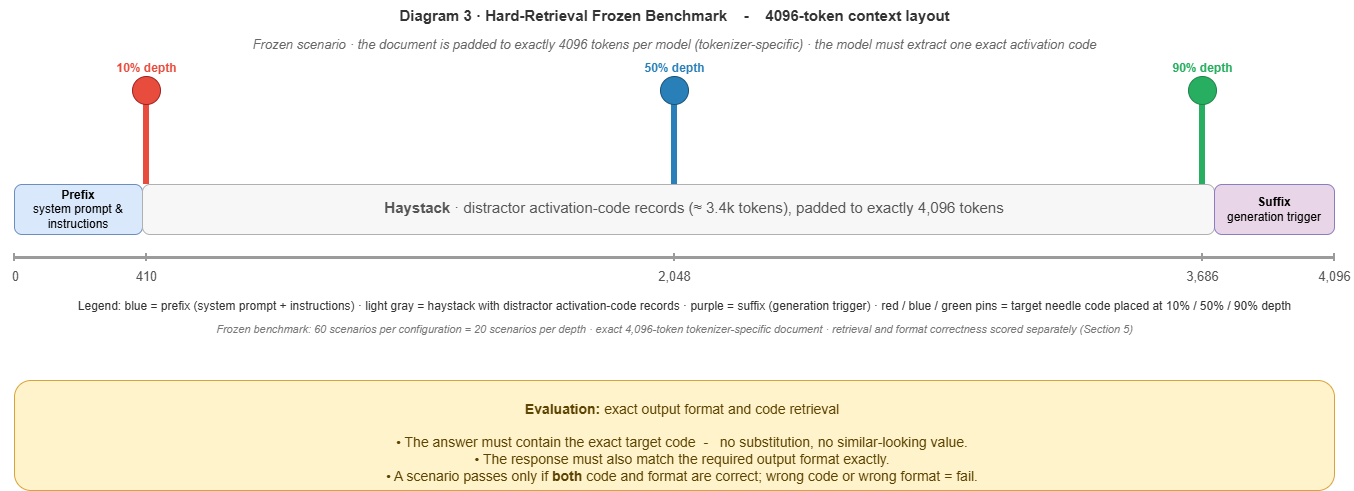
\includegraphics[width=0.72\columnwidth]{figures/hard_retrieval.png}
\Description{A 4096-token document diagram shows target-code needles inserted at 10, 50, and 90 percent depth within distractor text, with strict exact-match evaluation.}
\caption{Overview of the 4096-token hard-retrieval benchmark, showing the 10\%, 50\%, and 90\% depth needle insertion points within the distractor haystack, and the strict evaluation criteria.}
\label{fig:hard_retrieval}
\end{figure}

\subsection{Statistical Methodology}
Energy differences are evaluated using paired two-sided $t$-tests across five measurement blocks ($n=5$), reporting 95\% confidence intervals and controlling family-wise error rates with Holm sequential step-down correction~\cite{holm1979simple}. Non-parametric Wilcoxon signed-rank tests~\cite{wilcoxon1945individual} serve as secondary verification. Retrieval accuracy across 60 benchmark scenarios is reported with Wilson score 95\% confidence intervals~\cite{wilson1927probable}, and paired binary accuracy differences are tested via exact McNemar tests~\cite{mcnemar1947note} with Bonferroni correction. Cross-model retrieval contrasts and Pareto frontier stability are evaluated using depth-stratified bootstrap resampling over 2000 iterations.

%% ════════════════════════════════════════════════════════════════
%%  4. EMPIRICAL RESULTS
%% ════════════════════════════════════════════════════════════════
\section{Empirical Results}

\subsection{Energy and Decode Throughput Across Contexts}
\label{sec:energy-scaling}

Table~\ref{tab:energy-scaling} reports energy, decode throughput, peak allocated VRAM, and active KV-cache volume at each context length for both models.

\begin{table*}[t]
\caption{Total Energy (J, mean $\pm$ SD), Decode Throughput (tok/s), Peak Allocated VRAM (MiB), and Active Cache (MiB) Across Contexts}
\label{tab:energy-scaling}
\centering\small
\setlength{\tabcolsep}{4.5pt}
\resizebox{\textwidth}{!}{%
\begin{tabular}{@{}ll rrrr rrrr@{}}
\toprule
 & & \multicolumn{4}{c}{\textbf{Llama 3.2-3B (3:1 GQA)}} & \multicolumn{4}{c}{\textbf{Qwen2.5-3B (8:1 GQA)}} \\
\cmidrule(lr){3-6} \cmidrule(lr){7-10}
\textbf{Context} & \textbf{Configuration} & \textbf{Total Energy (J)} & \textbf{tok/s} & \textbf{Peak VRAM} & \textbf{Cache} & \textbf{Total Energy (J)} & \textbf{tok/s} & \textbf{Peak VRAM} & \textbf{Cache} \\
\midrule
1024 & FP16 Baseline (C0 / Q0)     & $244.11 \pm 13.10$ & 21.09 & 8810 & 119.0 & $258.57 \pm 27.40$ & 19.73 & 8061 & 38.2 \\
     & AWQ Baseline (C1-W / Q1-W)  & $268.77 \pm 26.20$ & 18.24 & 4943 & 119.0 & $293.42 \pm 21.61$ & 12.11 & 4273 & 38.2 \\
     & Eviction (C2 / Q2)          & $253.61 \pm 14.36$ & 19.31 & 4920 &  92.3 & $272.02 \pm 13.92$ & 12.91 & 4264 & 29.7 \\
     & TQ-Ref (C3-Ref / Q3-Ref)    & $367.00 \pm 28.44$ & 13.49 & 5099 & 187.2 & $358.58 \pm 9.61$  &  9.60 & 4321 & 60.2 \\
     & Compound (C4-Ref / Q4-Ref)  & $364.91 \pm 21.59$ & 12.75 & 5042 & 146.8 & $342.96 \pm 14.14$ &  9.76 & 4299 & 47.3 \\
\midrule
2048 & FP16 Baseline (C0 / Q0)     & $345.26 \pm 4.97$  & 17.42 & 9663 & 231.0 & $334.15 \pm 17.52$ & 17.87 & 8149 & 74.2 \\
     & AWQ Baseline (C1-W / Q1-W)  & $313.81 \pm 9.31$  & 20.13 & 5795 & 231.0 & $398.46 \pm 12.46$ & 13.70 & 4350 & 74.2 \\
     & Eviction (C2 / Q2)          & $338.74 \pm 21.03$ & 17.81 & 5691 & 119.0 & $342.56 \pm 10.34$ & 12.78 & 4297 & 38.2 \\
     & TQ-Ref (C3-Ref / Q3-Ref)    & $439.58 \pm 9.11$  & 13.33 & 6116 & 357.0 & $540.87 \pm 14.11$ &  8.94 & 4436 & 114.8 \\
     & Compound (C4-Ref / Q4-Ref)  & $435.05 \pm 24.47$ & 12.87 & 5853 & 187.2 & $435.18 \pm 20.00$ &  9.10 & 4343 & 60.2 \\
\midrule
4096 & FP16 Baseline (C0 / Q0)     & $701.08 \pm 8.12$  & 11.34 & 12688 & 455.0 & $616.78 \pm 6.79$  & 13.23 & 8249 & 146.2 \\
     & AWQ Baseline (C1-W / Q1-W)  & $631.25 \pm 5.05$  & 13.77 & 8820  & 455.0 & $621.75 \pm 25.14$ & 13.12 & 4460 & 146.2 \\
     & Eviction (C2 / Q2)          & $529.30 \pm 20.02$ & 20.34 & 8500  & 119.0 & $550.48 \pm 10.07$ & 12.53 & 4297 &  38.2 \\
     & TQ-Ref (C3-Ref / Q3-Ref)    & $913.48 \pm 2.11$  &  7.66 & 9468  & 696.5 & $812.28 \pm 13.11$ &  8.54 & 4668 & 223.9 \\
     & Compound (C4-Ref / Q4-Ref)  & $659.50 \pm 21.35$ & 12.53 & 8662  & 187.2 & $628.69 \pm 9.77$  &  9.04 & 4343 &  60.2 \\
\bottomrule
\end{tabular}}
\end{table*}

\paragraph{Context-Dependent AWQ Efficiency.}
On Llama, AWQ (C1-W) consumed 24.66~J more energy than uncompressed FP16 at 1024 tokens due to dequantization overhead on short sequences. However, at 4096 tokens, AWQ achieved a 9.96\% energy reduction (631.25~J vs.\ 701.08~J) as parameter bandwidth savings offset kernel overhead. On Qwen, AWQ did not yield energy savings over uncompressed FP16 at any context length (621.75~J vs.\ 616.78~J at 4096 tokens).

\paragraph{Long-Context Eviction Gains.}
At 4096 tokens on Llama, token eviction (C2) produced substantial multi-dimensional improvements over the AWQ baseline: reducing total energy by 101.95~J (16.15\%, 529.30~J vs.\ 631.25~J), accelerating decode throughput from 13.77 to 20.34~tok/s (47.7\% speedup), and cutting active cache volume by 73.8\% (455~MiB to 119~MiB).

\paragraph{Reference Quantization Overhead.}
TurboQuant reference (C3-Ref) increased energy consumption to 913.48~J on Llama (44.7\% over C1-W) and 812.28~J on Qwen (30.6\% over Q1-W) at 4096 tokens, while reducing throughput to 7.66 and 8.60~tok/s. Active cache memory expanded by over 50\% because the reference code retains uncompressed tensors alongside index tables.

\subsection{Llama Statistical Significance at 4096 Tokens}
Paired hypothesis tests for Llama total energy at 4096 tokens confirm that single-stage eviction (C2) significantly reduces energy over the AWQ baseline (C1-W) by $+101.95$~J (95\% CI: $[73.81, 130.08]$~J, Holm $p = 0.00549$), whereas TurboQuant reference (C3-Ref) imposes a significant penalty of $-282.24$~J ($[-287.23, -277.25]$~J, $p = 1.9 \times 10^{-7}$). Compound stacking (C4-Ref) does not differ significantly from the AWQ baseline ($-28.26$~J, $[-60.28, 3.76]$~J, $p = 0.2465$), but consumes significantly more energy than eviction alone ($-130.21$~J, $[-168.32, -92.09]$~J, $p = 0.00620$) and significantly less than standalone TurboQuant ($+253.98$~J, $[226.93, 281.02]$~J, $p = 0.000206$).

\subsection{Sequential Interaction and Overhead Shielding}
\label{sec:interaction}

To evaluate how multi-stage compression interacts when stacked sequentially, we define the interaction contrast:
\begin{equation}
I = (\text{C4-Ref} - \text{C3-Ref}) - (\text{C2} - \text{C1-W})
\end{equation}
A negative interaction ($I < 0$) indicates sub-additive energy consumption: the overhead of quantization is lower when applied after token eviction than when applied alone. For Llama, $I = -152.03$~J (95\% CI: $[-187.11, -116.96]$~J, $p = 0.00109$). Physically, eviction shrinks the active cache by 73.8\%, reducing the data volume processed by subsequent quantization routines during decoding. This negative interaction holds equally for Qwen ($I = -112.32$~J, 95\% CI: $[-151.78, -72.86]$~J, $p = 0.00352$) and remains invariant under power trace clipping at 82~W and 70~W.

\subsection{Hard-Retrieval Quality and Depth Analysis}

Table~\ref{tab:quality} reports exact-match retrieval accuracy across the 60 benchmark scenarios and broken down by needle insertion depth.

\begin{table}[t]
\caption{Hard-Retrieval Accuracy and Depth Breakdown at 4096 Tokens (60 Scenarios per Configuration)}
\label{tab:quality}
\centering\small
\setlength{\tabcolsep}{3.5pt}
\resizebox{\columnwidth}{!}{%
\begin{tabular}{@{}ll rrr rc@{}}
\toprule
\textbf{Model} & \textbf{Configuration} & \textbf{10\%} & \textbf{50\%} & \textbf{90\%} & \textbf{Pass/60} & \textbf{Wilson 95\% CI} \\
\midrule
Llama 3.2-3B   & FP16 Baseline (C0)     & 19/20 & 13/20 & 15/20 & 47/60 (78.3\%) & $[0.664,\ 0.869]$ \\
(3:1 GQA)      & AWQ Baseline (C1-W)    & 18/20 & 10/20 & 10/20 & 38/60 (63.3\%) & $[0.507,\ 0.744]$ \\
               & Eviction (C2)          & 18/20 & 10/20 &  9/20 & 37/60 (61.7\%) & $[0.490,\ 0.729]$ \\
               & TQ-Ref (C3-Ref)        & 18/20 & 10/20 &  9/20 & 37/60 (61.7\%) & $[0.490,\ 0.729]$ \\
               & Compound (C4-Ref)      & 17/20 & 10/20 & 10/20 & 37/60 (61.7\%) & $[0.490,\ 0.729]$ \\
\midrule
Qwen2.5-3B     & FP16 Baseline (Q0)     & 20/20 & 17/20 & 16/20 & 53/60 (88.3\%) & $[0.778,\ 0.942]$ \\
(8:1 GQA)      & AWQ Baseline (Q1-W)    & 18/20 & 15/20 & 15/20 & 48/60 (80.0\%) & $[0.682,\ 0.882]$ \\
               & Eviction (Q2)          &  0/20 &  0/20 &  1/20 &  1/60 (1.7\%)  & $[0.003,\ 0.089]$ \\
               & TQ-Ref (Q3-Ref)        & 18/20 & 16/20 & 15/20 & 49/60 (81.7\%) & $[0.701,\ 0.894]$ \\
               & Compound (Q4-Ref)      &  0/20 &  0/20 &  1/20 &  1/60 (1.7\%)  & $[0.003,\ 0.089]$ \\
\bottomrule
\end{tabular}}
\end{table}

\paragraph{Llama Retrieval Stability.}
On Llama, eviction (C2), TurboQuant (C3-Ref), and compound stacking (C4-Ref) each achieved 37/60 (61.7\%), differing from the AWQ baseline (38/60) by only a single test case (exact McNemar $p = 1.0$). Retrieval accuracy was highest at 10\% depth (17--18/20) and lower in the middle and end positions (9--10/20).

\paragraph{Qwen Eviction Collapse.}
On Qwen, single-stage eviction (Q2) caused retrieval accuracy to collapse to 1/60 (McNemar $p = 1.71 \times 10^{-13}$). Compound stacking (Q4-Ref) inherited this failure (1/60). Conversely, TurboQuant reference (Q3-Ref) preserved retrieval fidelity (49/60 vs.\ 48/60 on Q1-W). The cross-model eviction contrast $(\Delta_{\text{Qwen}} - \Delta_{\text{Llama}})$ was $-0.767$ (bootstrap 95\% CI: $[-0.867, -0.667]$).

\subsection{Qwen Sensitivity Sweeps}
Table~\ref{tab:qwen-sensitivity} summarizes sensitivity sweeps on Qwen at 4096 tokens. Increasing the eviction budget by 50\% (from 1024 to 1536 retained tokens) recovered only 2/15 scenarios, confirming that failure is driven by token selection errors under 8:1 GQA rather than capacity limits. In bit-width sweeps, 2-bit quantization caused notable accuracy loss (4/15), while 3-bit (11/15) and 4-bit (12/15) maintained accuracy.

\begin{table}[t]
\caption{Qwen Sensitivity Sweeps at 4096 Tokens (15 Common Test Scenarios)}
\label{tab:qwen-sensitivity}
\centering\small
\setlength{\tabcolsep}{4.5pt}
\resizebox{\columnwidth}{!}{%
\begin{tabular}{@{}l rrc@{}}
\toprule
\textbf{Variant} & \textbf{Total Energy (J)} & \textbf{Retrieval} & \textbf{Wilson 95\% CI} \\
\midrule
\multicolumn{4}{@{}l}{\textit{PyramidKV Token Budget Sweep:}} \\
Q2-B512 (Budget 512)   & $515.20 \pm 8.90$  & 0/15 & $[0.000,\ 0.218]$ \\
Q2-B1024 (Budget 1024) & $550.48 \pm 10.07$ & 1/15 & $[0.003,\ 0.234]$ \\
Q2-B1536 (Budget 1536) & $590.60 \pm 13.20$ & 2/15 & $[0.026,\ 0.320]$ \\
\midrule
\multicolumn{4}{@{}l}{\textit{TurboQuant Precision Sweep:}} \\
Q3-Ref-TQ2 (2-bit TQ)  & $808.90 \pm 34.00$ & 4/15  & $[0.109,\ 0.520]$ \\
Q3-Ref-TQ3 (3-bit TQ)  & $791.30 \pm 19.60$ & 11/15 & $[0.480,\ 0.891]$ \\
Q3-Ref-TQ4 (4-bit TQ)  & $812.28 \pm 13.11$ & 12/15 & $[0.548,\ 0.930]$ \\
\bottomrule
\end{tabular}}
\end{table}

\subsection{Multi-Objective Pareto Frontier and Bootstrap Stability}

Table~\ref{tab:pareto4d} shows the empirical four-objective Pareto frontier across total energy ($\min$), persistent KV cache footprint ($\min$), decode throughput ($\max$), and hard-retrieval accuracy ($\max$) at 4096 tokens, measured over 2000 paired bootstrap resamples. Figure~\ref{fig:pareto4d} shows the corresponding multi-objective trade-off profile using normalized parallel coordinates.

\begin{figure}[t]
\centering
\begin{subfigure}{\columnwidth}
  \centering
  \includegraphics[width=\linewidth,trim=0 28bp 445.8bp 20bp,clip]{figures/fig_pareto_4d_parallel_coords.pdf}
  \caption{Llama~3.2-3B (3:1 GQA).}
\end{subfigure}
\vspace{-2pt}
\begin{subfigure}{\columnwidth}
  \centering
  \includegraphics[width=\linewidth,trim=445.8bp 28bp 0 20bp,clip]{figures/fig_pareto_4d_parallel_coords.pdf}
  \caption{Qwen2.5-3B (8:1 GQA).}
\end{subfigure}
\vspace{1pt}

{\scriptsize
\begin{tabular}{@{}lllll@{}}
\textcolor[HTML]{4C78A8}{\rule{7pt}{1.2pt}} FP16 &
\textcolor[HTML]{2A9D8F}{\rule{7pt}{1.2pt}} AWQ &
\textcolor[HTML]{F28E2B}{\rule{7pt}{1.2pt}} Eviction &
\textcolor[HTML]{8064A2}{\rule{7pt}{1.2pt}} TQ-Ref &
\textcolor[HTML]{C7A9E8}{\rule{7pt}{1.2pt}} Evict.+TQ-Ref
\end{tabular}}
\Description{Four-axis parallel coordinates plot comparing energy, memory, throughput, and retrieval accuracy for Llama and Qwen.}
\caption{Four-axis parallel coordinates trade-off profile at 4096 tokens across total energy, KV cache footprint, decode throughput, and hard-retrieval accuracy. Solid polylines indicate four-dimensional Pareto-optimal configurations, and dashed polylines denote dominated configurations.}
\label{fig:pareto4d}
\end{figure}

\begin{table}[t]
\caption{Four-Objective Pareto Frontier Analysis at 4096 Tokens (2000 Bootstrap Resamples)}
\label{tab:pareto4d}
\centering\scriptsize
\setlength{\tabcolsep}{2.5pt}
\resizebox{\columnwidth}{!}{%
\begin{tabular}{@{}ll rrr cc@{}}
\toprule
\textbf{Model} & \textbf{Config} & \textbf{Energy (J) $\downarrow$} & \textbf{Cache (MiB) $\downarrow$} & \textbf{tok/s $\uparrow$} & \textbf{Retrieval $\uparrow$} & \textbf{Viable ($Q \ge 50\%$)} \\
\midrule
Llama 3.2-3B   & FP16 (C0)            & $701.08 \pm 8.12$  & 455.0 & $11.34 \pm 0.06$ & 0.783 (47/60) & \textbf{Yes} (100.0\%) \\
               & AWQ Baseline (C1-W)  & $639.86 \pm 5.48$  & 455.0 & $13.71 \pm 0.24$ & 0.633 (38/60) & \textbf{Yes} (63.3\%) \\
               & AWQ + Evict (C2)     & $529.30 \pm 20.02$ & 119.0 & $20.34 \pm 1.62$ & 0.617 (37/60) & \textbf{Yes} (100.0\%) \\
               & AWQ + TQ-Ref (C3-Ref)& $913.48 \pm 2.11$  & 696.5 &  $7.66 \pm 0.02$ & 0.617 (37/60) & No (Dominated) \\
               & Compound (C4-Ref)    & $659.50 \pm 21.35$ & 187.2 & $12.53 \pm 0.96$ & 0.617 (37/60) & No (Dominated) \\
\midrule
Qwen2.5-3B     & FP16 (Q0)            & $616.78 \pm 6.79$  & 146.2 & $13.23 \pm 0.15$ & 0.883 (53/60) & \textbf{Yes} (97.9\%) \\
               & AWQ Baseline (Q1-W)  & $621.75 \pm 25.14$ & 146.2 & $13.12 \pm 1.03$ & 0.800 (48/60) & No (Dominated) \\
               & AWQ + Evict (Q2)     & $550.48 \pm 10.07$ &  38.2 & $12.53 \pm 1.46$ & 0.017 (1/60)  & \xmark\ (Failed $Q$) \\
               & AWQ + TQ-Ref (Q3-Ref)& $812.28 \pm 13.11$ & 223.9 &  $8.60 \pm 0.37$ & 0.817 (49/60) & No (Dominated) \\
               & Compound (Q4-Ref)    & $628.69 \pm 9.77$  &  60.2 &  $9.04 \pm 0.60$ & 0.017 (1/60)  & \xmark\ (Failed $Q$) \\
\bottomrule
\end{tabular}}
\end{table}

For Llama, single-stage eviction (C2) provides the most favorable balance across system metrics: minimal total energy ($529.30\pm 20.02$~J), smallest cache footprint ($119.0$~MiB), and maximal throughput ($20.34\pm 1.62$~tok/s), while staying within one test case of the baseline retrieval rate (37/60 vs.\ 38/60, $61.7\%$ vs.\ $63.3\%$) with 100.0\% bootstrap selection stability. Uncompressed FP16 (C0, 100.0\%) and stock AWQ (C1-W, 63.3\%) remain on the Pareto frontier due to better retrieval accuracy (78.3\% and 63.3\%). TurboQuant reference variants C3-Ref (0.0\%) and C4-Ref (36.2\%) are dominated. Crucially,Eviction  (C2) strictly outperforms compound stack (C4-Ref) across all operational conditions (19.7\% lower energy, 62.3\% higher throughput, 36.4\% smaller cache at identical 37/60 retrieval), showing that sequential stacking introduces unnecessary overhead compared to single-stage eviction on balanced attention geometry.

For Qwen, the Pareto analysis reveals a sharp split. Uncompressed FP16 (Q0) is Pareto-optimal ($616.78\pm 6.79$~J, $13.23$~tok/s, 88.3\% retrieval, 97.9\% bootstrap stability), strictly dominating stock AWQ (Q1-W, $621.75$~J, 80.0\% retrieval). Token eviction (Q2) achieves 100.0\% unconstrained bootstrap selection on energy ($550.48$~J) and memory ($38.2$~MiB) alone, but drops retrieval accuracy to $1/60$ (1.7\%). When filtered by a practical operational threshold ($Q \ge 50\%$), Q2 (Eviction) is excluded as non-viable, leaving Q0 (Baseline) as the sole viable frontier configuration.

\subsection{Power Trace Robustness}
\label{sec:robustness}
Raw NVML power traces feature transient excursions above nominal 70~W values, with isolated samples exceeding 100~W (peaking at 124.5~W on Llama and 116.1~W on Qwen). To confirm that our findings are not artifacts of measurement spikes, we reintegrated all power traces with an 82~W cap and a strict 70~W cap. All five registered statistical significance decisions and the energy rank ordering ($\text{Evict} < \text{AWQ} < \text{Compound} < \text{FP16} < \text{TQ-Ref}$) remained unchanged.

%% ════════════════════════════════════════════════════════════════
%%  5. DISCUSSION AND LIMITATIONS
%% ════════════════════════════════════════════════════════════════
\section{Discussion and Limitations}

\subsection{Divergence Between Expectations and Empirical Findings}
Existing research suggests that the combination of weight quantization, token eviction, and KV-cache compression should enable multiplicative improvements in energy and memory footprint while maintaining task performance. However, these expectations were challenged by our empirical findings: \textbf{(1) AWQ Baseline:} Saves $\approx 10\%$ energy on Llama at 4096 tokens, but increases energy at 1024 tokens and yields no net savings on Qwen; \textbf{(2) TurboQuant Reference:} Realized reference package expanded physical DRAM storage by over 50\% and added 31\% to 45\% energy overhead; \textbf{(3) Eviction Portability:} Preserved retrieval on Llama (37/60), but collapsed on Qwen (1/60); and \textbf{(4) Compound Stacking:} Compound stacking (C4-Ref) was not significantly lower than AWQ (C1-W) and collapsed to 1/60 on Qwen. This shows that nominal compression ratios in theory do not always translate into practice when KV-cache tensors are kept uncompressed in software and sensitive attention layouts are involved.

\subsection{Eviction Divergence and Architecture Sensitivity}
The largest difference in our data is the difference in retrieval outcomes under token eviction. This can be explained by architectural differences between Llama~3.2-3B and Qwen2.5-3B: \textbf{(1) GQA Head Sharing:} Qwen has an 8:1 query-to-KV head ratio (16 query heads sharing 2 KV heads), while Llama has a 3:1 ratio (24 query heads sharing 8 KV heads). In an 8:1 configuration, evicting one KV token removes historical context from eight query heads simultaneously; \textbf{(2) Tokenization Density:} Differences in vocabulary and chat formatting shift relevant information relative to layer attention windows; and \textbf{(3) Heuristic Portability:} Attention-based importance heuristics, primarily developed on balanced GQA structures, do not transfer reliably to aggressive head sharing.

\begin{figure}[t]
\centering
\begin{subfigure}{\columnwidth}
  \centering
  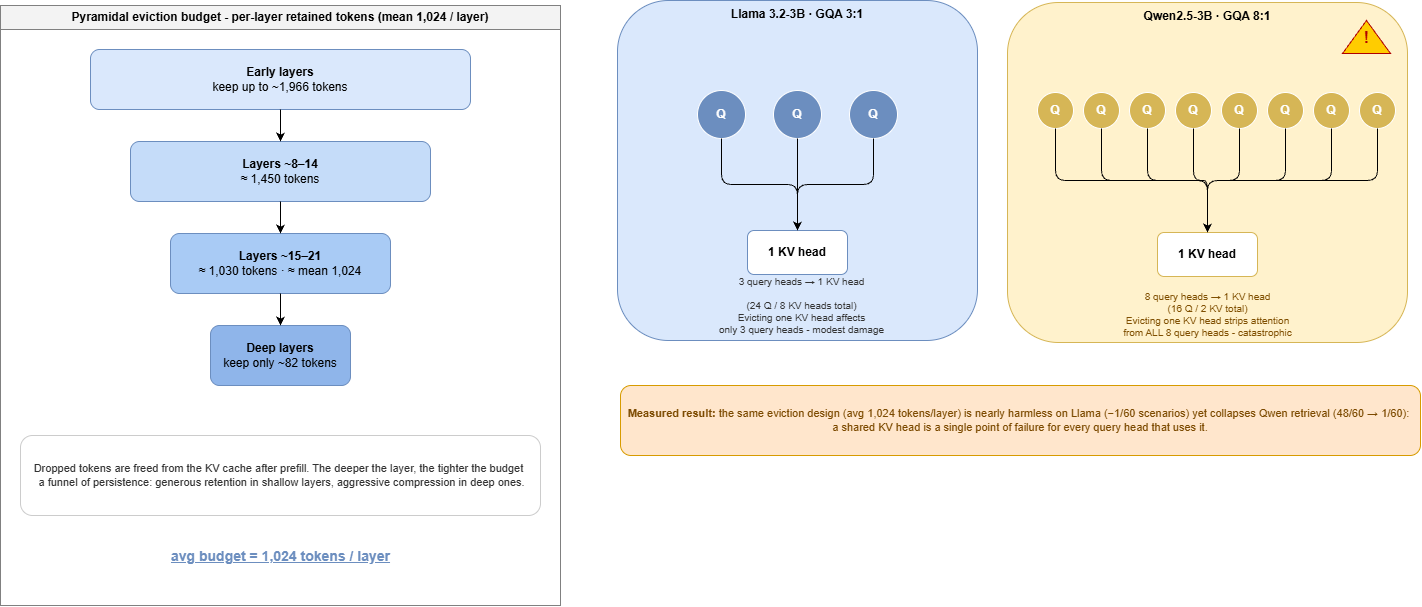
\includegraphics[width=0.70\linewidth,trim=0 0 850bp 0,clip]{figures/eviction_graph.png}
  \caption{Layerwise pyramidal token budgets.}
\end{subfigure}
\vspace{-4pt}
\begin{subfigure}{\columnwidth}
  \centering
  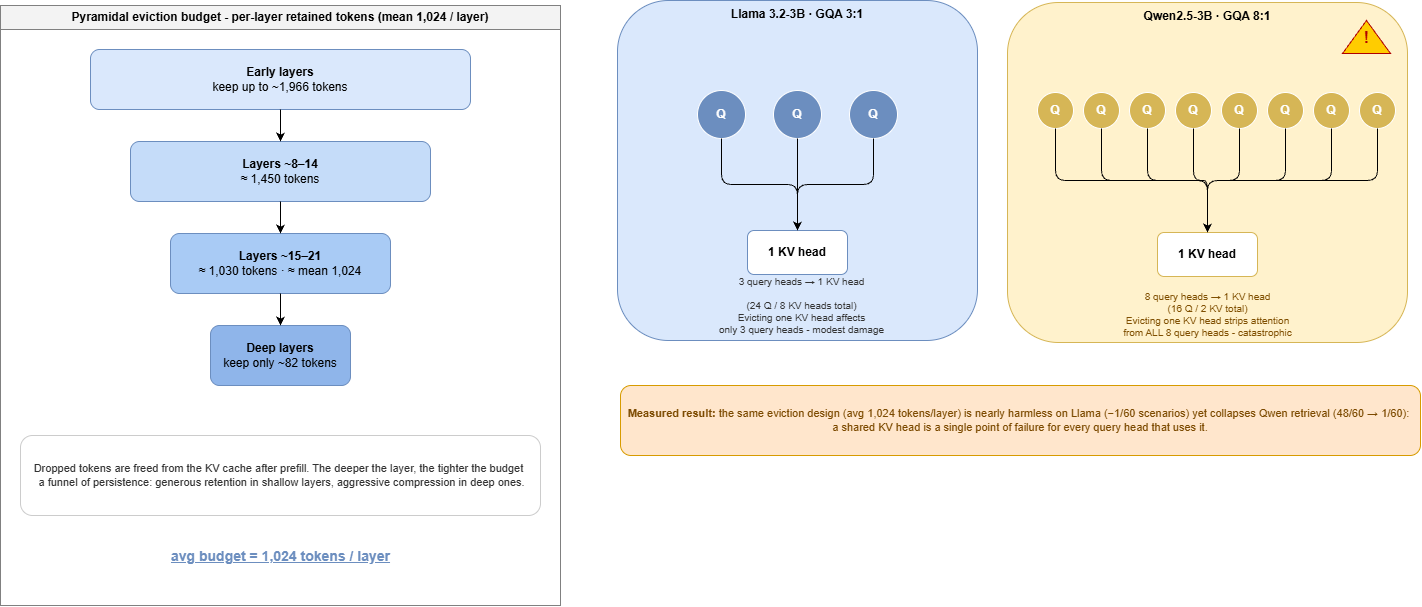
\includegraphics[width=0.80\linewidth,trim=620bp 0 0 0,clip]{figures/eviction_graph.png}
  \caption{Grouped-query attention layouts.}
\end{subfigure}
\Description{A diagram compares pyramidal eviction budgets and grouped-query attention geometry between Llama and Qwen.}
\caption{PyramidKV budgets and GQA head-sharing layouts. Under Qwen's 8:1 ratio, removing one KV token simultaneously removes context from eight query heads, causing more severe retrieval degradation than in Llama's 3:1 layout.}
\label{fig:eviction_gqa}
\end{figure}

Importantly, our empirical sensitivity sweep rules out simple hyperparameter capacity mismatch as the root cause: increasing the average retained token budget by 50\% (from 1024 to 1536 tokens, Table~\ref{tab:qwen-sensitivity}) recovered only two additional scenarios (2/15 pass rate). This confirms that the retrieval collapse is due to errors in structural token selection under 8:1 GQA, rather than a lack of memory capacity. Figure~\ref{fig:eviction_gqa} illustrates how GQA geometry amplifies the impact of token removal.

\subsection{Physical Execution versus Nominal Compression}
We evaluate TurboQuant over a numerical reference implementation rather than an optimized fused kernel. A production kernel that physically packs coordinate indices and fuses dequantization directly into attention compute could approach ideal memory targets (reducing decode cache down to 28.8\% of FP16 at 4 bits). Reporting measured execution characteristics provides an empirical baseline for future kernel development.

\subsection{Scope of Statistical Claims}
\paragraph{Established Empirical Findings.}
The registered experimental matrix establishes: (1) token eviction significantly reduces total energy consumption on Llama at 4096 tokens (Holm $p = 0.00549$); (2) the TurboQuant reference package significantly increases total energy consumption across both models; (3) both models exhibit a statistically significant negative interaction ($I < 0, p < 0.01$), confirming that prior eviction reduces quantization workload; (4) token eviction severely degraded hard-retrieval performance on Qwen ($p = 1.71 \times 10^{-13}$); and (5) energy rankings and significance decisions were stable under clipping of power traces at 82~W and 70~W.

\paragraph{Boundaries and Non-Claims.}
Conversely, the data does not establish: (1) strict energetic equivalence between AWQ baseline (C1-W) and compound stacking (C4-Ref) (the 95\% CI $[-60.28, 3.76]$~J spans zero but remains wide); (2) that Qwen's retrieval failure was caused solely by GQA geometry to the exclusion of tokenization or attention patterns; (3) that energy penalties in the reference implementation would persist in a custom fused CUDA kernel; (4) that Llama's retrieval retention generalizes to context lengths larger than 4096 tokens or open-ended reasoning tasks; or (5) that AWQ provides stable energy savings across all sequence lengths.

\subsection{Bridging Sequential Stacking and Joint Optimization (RDKV and ThinKV)}
\label{sec:joint-opt}
Our empirical results provide direct physical motivation for the flourishing literature on joint rate-distortion compression. Theoretical frameworks such as \textbf{RDKV}~\cite{zhang_rdkv_2026} and \textbf{ThinKV}~\cite{ramachandran_thinkv_2026} explore continuous bit allocation for tokens and layers dynamically, where token eviction is considered as a special case of zero-bit assignment in a rate-distortion objective.

While these frameworks generate promising Pareto frontiers in algorithmic simulation, our hardware measurements show tangible failure modes of disjoint sequential pipelines which demand joint optimization on real devices. As empirically illustrated by our Pareto frontier, naive sequential compound stacking (C4-Ref) is strictly behind single-stage eviction (C2) on balanced architectures like Llama, and leads to complete retrieval collapse (1/60) on aggressive head-sharing layouts like Qwen. The physical silicon results present boundary conditions for RDKV and ThinKV: to preserve directional attention signals, marginal tokens have to be kept at low precision (1 or 2 bits) under aggressive GQA, since hard binary eviction discards them. Our measurement of the sequential shielding effect ($I < 0$) confirms that shrinking active cache volume prior to quantization yields genuine energy savings by reducing DRAM read traffic.

\subsection{Limitations and Threats to Validity}
\paragraph{Internal and Construct Validity.} All measurements were collected within continuous sessions on Google Colab with 5 independent blocks per condition ($n=5$). Quantized Llama variants were evaluated with the attention wrapper applied, introducing a minor baseline shift ($\approx 8.61$~J at 4096 tokens). On Qwen, the wrapper was applied consistently across all configurations. All trace files were verified with SHA-256 checksums. Retrieval quality is measured with exact-match key-value extraction at three document depths; while this isolates memory retention, it does not assess multi-step reasoning or dialogue. Power measurements capture board-level GPU dissipation with NVML, excluding host CPU and system RAM.
\paragraph{External and Statistical Validity.} Experiments used two open-weight 3B models on an NVIDIA T4 GPU. Because Llama and Qwen differ in layer counts (28 vs.\ 36) and vocabulary tokenization (128k vs.\ 152k) alongside GQA ratios (3:1 vs.\ 8:1), GQA is the primary structural factor but is not completely isolated from other architectural differences. Fixed 64-token decoding isolates compression mechanisms but does not model variable-length dialogue. Family-wise error rates were controlled using Holm correction for energy contrasts and Bonferroni adjustments for McNemar tests. Wilson score intervals quantify binomial uncertainty at $n=60$, and bootstrap resampling quantifies Pareto selection stability.

%% ════════════════════════════════════════════════════════════════
%%  6. CONCLUSION AND REPRODUCIBILITY
%% ════════════════════════════════════════════════════════════════
\section{Conclusion and Reproducibility}

This paper presented an empirical systems ablation of multi-stage compression on two 3B-parameter small language models running on an NVIDIA T4 GPU. We measured 10~Hz power traces up to 4096 tokens and calculated retrieval accuracy using a calibrated 60-scenario benchmark.

Our primary finding is that compression efficiency depends on attention head layout and sequence length, not nominal compression ratios alone. On Llama~3.2-3B (3:1 GQA), combining 4-bit AWQ with PyramidKV eviction delivered a 101.95~J (16.15\%) energy reduction, a 47.7\% throughput speedup, a 73.8\% smaller active cache, and retrieval accuracy matching baseline (37/60 vs.\ 38/60). On Qwen2.5-3B (8:1 GQA), the same eviction heuristic collapsed accuracy to 1/60. We also confirmed a negative compound interaction ($I < 0, p < 0.01$), showing that upstream eviction shields against downstream quantizer overhead. These results provide empirical boundary conditions for theoretical joint rate-distortion compression on edge accelerators.

To support complete reproducibility, all experimental protocols, model checkpoints, raw 10~Hz NVML power traces, benchmark scenarios, evaluation scripts, and synthesis notebooks will be made publicly available upon publication. Table~\ref{tab:reproducibility-specs} summarizes the execution environment and specifications.

\begin{table}[t]
\caption{Reproducibility Environment and Execution Parameters}
\label{tab:reproducibility-specs}
\centering\footnotesize
\setlength{\tabcolsep}{2pt}
\resizebox{\columnwidth}{!}{%
\begin{tabular}{@{}ll@{}}
\toprule
\textbf{Category} & \textbf{Configuration / Specification} \\
\midrule
Hardware & NVIDIA Tesla T4 (Turing, 40 SMs, 16~GB VRAM, 70~W cap) \\
Host System & Linux x86\_64 (kernel 6.6.122+), Intel Xeon CPU @ 2.00~GHz \\
Software Stack & PyTorch 2.11.0+cu128, Transformers 5.12.1, CUDA 12.8 \\
Quantization & \texttt{gptqmodel==7.1.0}, \texttt{turboquant==0.2.0} \\
Power Sampling & 10~Hz via NVML (\texttt{pynvml}), trapezoidal $\int P(t)\,dt$ \\
Models & Llama~3.2-3B-Instruct (3:1 GQA), Qwen2.5-3B-Instruct (8:1 GQA) \\
Eviction Policy & Custom PyramidKV (decay $\beta=20$, win 32, budget avg 1024) \\
Benchmark & Calibrated hard-retrieval NIAH UUID extraction (60 scenarios) \\
Contexts & 1024, 2048, 4096 tokens (64-token greedy decode, $n=5$ runs) \\
\bottomrule
\end{tabular}}
\end{table}

%% ════════════════════════════════════════════════════════════════
%%  ACKNOWLEDGMENTS
%% ════════════════════════════════════════════════════════════════
\section*{Acknowledgments}
Generative AI was used minimally to assist with LaTeX formatting and document structuring. It was not used in the study design or in generating, interpreting, or analyzing the research findings or scientific content. The authors take full responsibility for the content and integrity of the publication.

%% ════════════════════════════════════════════════════════════════
%%  REFERENCES
%% ════════════════════════════════════════════════════════════════
\bibliographystyle{ACM-Reference-Format}
\begingroup
\footnotesize
\sloppy
\hbadness=10000
\setlength{\bibsep}{0.5pt plus 0.2pt minus 0.2pt}
\bibliography{references}
\endgroup

\end{document}
